\chapter{Grundlagen}

\section{Assembler}

Assembler ist eine Programmiersprache der zweiten Generation und ist ein direkter Nachfolger der Programmierung in Maschinensprache, also mit Zahlencodes. Bei Assembler handelt es sich um eine hardwarenahe Programmiersprache. Je nachdem welche Hardware verwendet wird, stehen unterschiedliche Befehlssätze zur Verfügung. Daher gibt es nicht die \zitat{eine} Programmiersprache Assembler, sondern es handelt sich um eine Gruppe von Assemblersprachen, die für die jeweilige Hardware angepasst ist.\cite{bib:assembler}

Generell handelt es sich bei Assembler um eine zeilenorientierte Sprachfamilie, das heißt eine Zeile stellt immer eine komplette Anweisung dar. Diese Anweisungen bestehen aus den hardware-spezifischen Befehlen.\cite{bib:assembler_book}

\section{Der 8051 Mikrocomputer} \label{section:8051}

Der 8051 Mikrocomputer wurde 1981 von Intel als 8-bit Mikrocontroller auf den Markt gebracht. Es handelt sich um ein \zitat{system on a chip}, was bedeutet, dass RAM, ROM, zwei Timer, ein Serial Port, 4 8-bit Ports und noch einiges mehr auf einem einzigen Chip verbaut sind. Die einzelnen Bestandteile sind in Abbildung \ref{img:8051} dargestellt.\cite{bib:8051} 

Mittlerweile ist der Original 8051 veraltet, dennoch existieren viele Abwandlungen (Derivate) beziehungsweise Weiterentwicklungen des 8051. Diese sind allerdings mit höherer Taktfrequenz und geringerer Taktteilung ausgestattet, sodass sie nahezu auf dem aktuellen Stand der Technik und damit deutlich leistungsfähiger als das Ursprungsmodell sind.\cite{bib:8051_2}

\begin{figure}[htbp]
	\centering
	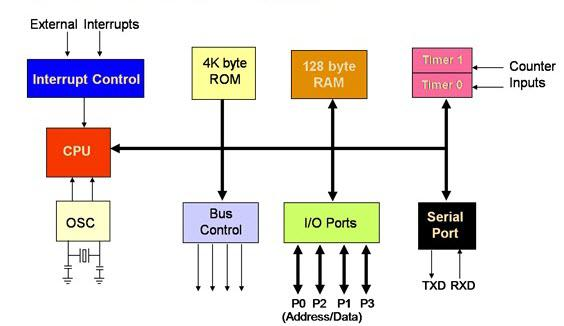
\includegraphics[scale=0.75]{img/8051-diagram}
	\caption{Blockdiagramm eines 8051 Mikrocomputers}
	\label{img:8051}
	\source{https://www.tutorialspoint.com/embedded_systems/images/block_diagram.jpg}
\end{figure}


\section{Entwicklungsumgebung MCU-8051 IDE} \label{section:ide}

Die MCU-8051 IDE ist eine integrierte Entwicklungsumgebung für Mikrocontroller und basiert auf dem 8051 Mikroprozessor. Neben Assembler können die Programme auch in C entwickelt werden.

Die IDE unterstützt den Entwicklungsprozess neben einem Quellcode Editor auch mit einem Simulator zum direkten Ausführen des Programms auf verschiedenen Mikrocontrollern. Auch eine Hardware-Anbindung in Form eines LCD Displays, eines Keypads und vielen weiteren Tools wird von der MCU-8051 IDE bereitgestellt.\cite{bib:mcu}